\def\angle{0}
\def\radius{3}
\def\cyclelist{{"blue","red","green","green"}}
\newcount\cyclecount \cyclecount=-1
\newcount\ind \ind=-1
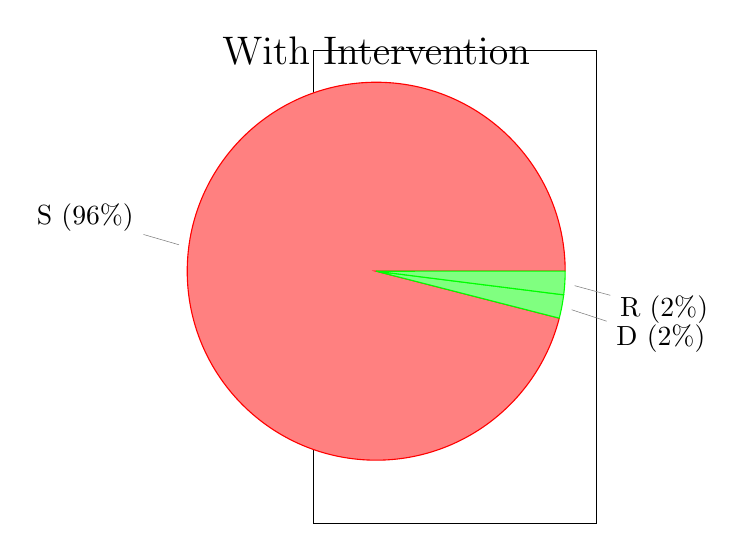
\begin{tikzpicture}[scale=.8]
\draw[white] (-1,-4) rectangle (3.5,3.5);
\node at (0,3.5) {\Large With Intervention};
  \foreach \percent/\name in {
      96/S (96\%),
      2/D (2\%),
      2/R (2\%)
    } {
      \ifx\percent\empty\else               % If \percent is empty, do nothing
        \global\advance\cyclecount by 1     % Advance cyclecount
        \global\advance\ind by 1            % Advance list index
        \ifnum3<\cyclecount                 % If cyclecount is larger than list
          \global\cyclecount=0              %   reset cyclecount and
          \global\ind=0                     %   reset list index
        \fi
        \pgfmathparse{\cyclelist[\the\ind]} % Get color from cycle list
        \edef\color{\pgfmathresult}         %   and store as \color
        % Draw angle and set labels
        \draw[fill={\color!50},draw={\color}] (0,0) -- (\angle:\radius)
          arc (\angle:\angle+\percent*3.6:\radius) -- cycle;
        %\node at (\angle+0.5*\percent*3.6:0.85*\radius) {\percent\,\%};
        \node[pin=\angle+0.5*\percent*3.6:\name]
          at (\angle+0.5*\percent*3.6:\radius) {};
        \pgfmathparse{\angle+\percent*3.6}  % Advance angle
        \xdef\angle{\pgfmathresult}         %   and store in \angle
      \fi
    };
\end{tikzpicture}
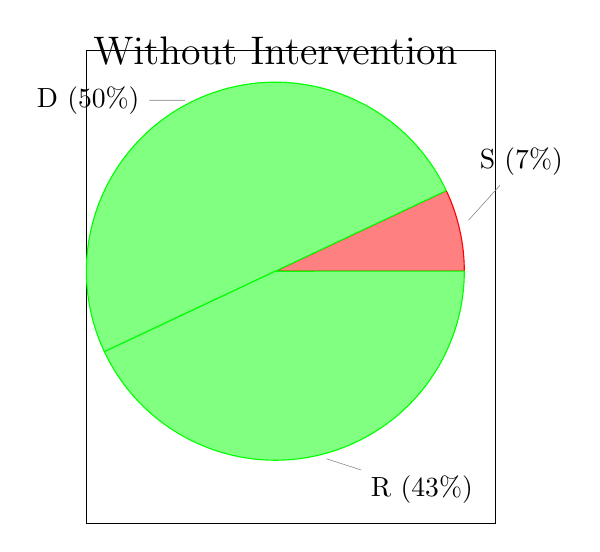
\begin{tikzpicture}[scale=.8]
\draw[white] (-3,-4) rectangle (3.5,3.5);
	\node at (0,3.5) {\Large Without Intervention};
  \foreach \percent/\name in {
      7/S (7\%),
      50/D (50\%),
      43/R (43\%)
    } {
      \ifx\percent\empty\else               % If \percent is empty, do nothing
        \global\advance\cyclecount by 1     % Advance cyclecount
        \global\advance\ind by 1            % Advance list index
        \ifnum3<\cyclecount                 % If cyclecount is larger than list
          \global\cyclecount=0              %   reset cyclecount and
          \global\ind=0                     %   reset list index
        \fi
        \pgfmathparse{\cyclelist[\the\ind]} % Get color from cycle list
        \edef\color{\pgfmathresult}         %   and store as \color
        % Draw angle and set labels
        \draw[fill={\color!50},draw={\color}] (0,0) -- (\angle:\radius)
          arc (\angle:\angle+\percent*3.6:\radius) -- cycle;
        %\node at (\angle+0.5*\percent*3.6:0.85*\radius) {\percent\,\%};
        \node[pin=\angle+65+0.5*\percent*3.6:\name]
          at (\angle+0.5*\percent*3.6:\radius) {};
        \pgfmathparse{\angle+\percent*3.6}  % Advance angle
        \xdef\angle{\pgfmathresult}         %   and store in \angle
      \fi
    };
\end{tikzpicture}